\documentclass[11pt]{article}

\usepackage{changepage}
\usepackage{amsmath}
\usepackage[a4paper, total={7.25in, 10in}]{geometry}
\usepackage{url}
\usepackage{indentfirst}
\usepackage{hanging}
\usepackage[document]{ragged2e}
\usepackage[notes, short, backend=biber]{biblatex-chicago}
\usepackage{cmsendnotes}
\usepackage{graphicx}
\usepackage{hyperref}

\addbibresource{./4-delicacy-part-one.bib}
\setlength{\parindent}{0pt}
\setlength{\RaggedRightParindent}{0pt}
\setlength{\parskip}{1em}

\newcommand{\BExcerpt}{}
\newcommand{\EExcerpt}{}

\title{delicacy part one}
\date{8 December 2024}

\begin{document}
    \maketitle
    April 2023 saw the publication of Hadley Freeman's \textit{Good Girls: A Story and Study of Anorexia}, a memoir recounting her experience with anorexia in her teenage years. It was generally positively-reviewed, with \textit{The Guardian} calling it ``a clear-eyed view of a debilitation and misunderstood illness.''~\footfullcite{Guardian23} More notable is the ``study'' part of this ``story and study'' -- discussing \textit{Good Girls} for \textit{The Telegraph} in one of very few critical reviews, medical humanities scholar Emma Seaber wrote: ``The book contains numerous errors. Some are trivial; others gross distortions.''~\footfullcite{Telegraph23} 

    Seaber expounds on these errors in a blog post, detailing the many ``omissions, exaggerations, misleading stuff, [and] lazy research.'' Freeman equates alcohol use among those with anorexia or bulimia to alcohol abuse, suggests that less than 0.1\% of anorexia cases begin in adulthood (when, in reality, around 40\% do), and misrepresents the cause of Karen Carpenter's death.~\footfullcite{Seaber23a} I would like to investigate, though, a comparison Seaber makes in her published review between Freeman's book and late twentieth century feminist works by the likes of Susie Orbach, Kim Chernin, and Susan Bordo that postulate eating disorders less as pathologies and more as products of troubled femininity.

    Of these works, the latter is the furthest-reaching.
    \BExcerpt
    Posited as a new discipline of ``body studies,'' Susan Bordo's \textit{Unbearable Weight: Feminism, Western Culture, and the Body} attempts to read eating disorders, particularly anorexia and bulimia, as physical manifestations, on the ``text'' of the body, of various cultural influences. It received nearly universal praise upon its release, both as a ``detailed, nuanced, and generally well-written'' analysis of ``various women's experiences'' of eating disorders and as a more theoretical work concerning ``the body's materiality'' and its importance in feminist discourse. Far from the relic of the 1990s that this might suggest it to be, \textit{Unbearable Weight} has been cited, over twelve thousand times (almost four hundred times in 2022 alone). Excerpts have appeared in at least nineteen anthologies; I first encountered it as an undergrad in the influential \textit{Norton Anthology of Theory and Criticism} where, as in the reviews in \textit{Discourse} and \textit{Hypatia}, it was positioned as a popular, accessible, American response to apparently academic, impenetrable, French feminism. Criticism of Bordo's work that fell outside this disagreement on theory was sparse if present at all, usually remarking on the arrangement of essays being noncohesive.~\autocites[176]{Green94}[153]{Hekman95}
    \EExcerpt
    
    To quickly help situate us, I'll start by summarizing some of her theoretical goals and methods. She starts from the observation that ``certain cultural images and ideology'' are responsible for both interpersonal and internalized gender stereotypes, most significantly an association of femininity with passivity and the ``degraded'' body, contrasted with masculinity and its autonomy and ``will.''~\autocite[16.3]{Bordo03} Referencing Foucault, she sees this ``gender ideology'' as part of a web of cultural power that crystallizes in demands placed upon the bodies of individuals. For her, anorexia and bulimia in women are physical results of this opposition between passivity and autonomy, and that this ``cultural evidence is so overwhelming'' as to render irrelevant posited ``biological explanations,'' which she calls ``blind allegiance to the medical model.'' While psychiatric study of eating disorders frequently includes cultural considerations, Bordo rejects that they demonstrate a ``pathogenic situation'' explainable by ``biological, psychological, [or] familial'' means.~\autocite[35, 49]{Bordo03} 

    The book is divided into three parts. The first, ``Discourses and Conceptions of the Body,'' compares Bordo's own cultural theory of eating disorders with the so-called ``medical model'' and speculates about the effects of various contemporary media images related to food, eating, and hunger, with an interlude on the politics of motherhood and pregnancy. The second part, ``The Slender Body and Other Cultural Forms,'' attempts to explain further her theoretical framework, as well as to establish a historically-consistent symbology of fatness and thinness. The final part, ``Postmodern Bodies,'' begins with a criticism of other, in her opinion postmodern, feminist theories alongside a justification of her own theory of gender, before returning to the same sort of analysis of pop culture depictions of people's bodies. 
    
    \subsection*{Medicine and superwomen}

    Since \textit{Unbearable Weight}'s first claim to authority is the relative insufficiency of medicine in understanding eating disorders, we might start by analyzing Bordo's relationship with medicine. Since it has been over thirty years since the book's first publication, it is predicable that many of Bordo's characterizations of medicine, in particular the statistics she shares, are no longer accurate. More recent research into eating disorders should cause us to notice, for instance, Bordo's repeated declaration that ``initially, anorexia was found to predominate among upper-class white families.'' This claim is alongside one that ``approximately 90 percent of sufferers are girls or women.''~\autocite[50]{Bordo03} Neither of these are supported by evidence today, where current research shows that as many as 25\% of people with anorexia or bulimia are male, and that the ratio of males to females diagnosed changes over time, with some studies reporting a ratio as high as 0.5 in the United States.~\autocite[1409]{Galmiche19} She does follow these observations by noting that the demographics of anorexia are ``rapidly changing'' due to ``the power of popular imagery,'' a sentiment she repeats in the preface to the tenth anniversary edition as an example of the predictive power of her work.~\autocite[320]{Bordo03} However, this technique of explaining demographic shifts is somewhat suspect -- while it is certainly possible that everything occurred in accordance with Bordo's theories, it says nothing about the relative accuracy of her sources. Demographic reports about the prevalence of anorexia have changed dramatically since 1993 -- one explanation is that anorexia has spread like a disease, a cultural contagion infecting more and more people. Another, and in my opinion more likely, explanation is that medical and especially psychological scientific methods have also changed dramatically since 1993, as have the diagnostic criteria for these disorders. While we'll evaluate the relative merits of both explanations, we have to remember from the outset that the cultural apparatus posited in \textit{Unbearable Weight} can't possibly be used to support the correctness of the statistical data upon which it's predicated.  
    
    Even so, judging the validity of Bordo's quantitative data is fraught -- \textit{Unbearable Weight} is not a work of science (nor does it intend to be). It does not have a coherent methodology; its statistical sources are syncretically assembled from various memoirs, psychology studies, personal accounts, and magazine articles. In her treatment of the studies, she frequently quotes isolated sentences that were published in journals of varying repute, but leaves it to us to learn more about the studies in question. What were their stated aims and methodologies? What populations did they sample? What conclusions did the authors themselves draw from this data? 
    
    So, early on, Bordo introduces us to Catherine Steiner-Adair's ``provocative study of high-school women which revealed a striking association between problems with food and body image and emulation of the beautiful, independent, cool superwoman of media imagery.''~\autocite[47]{Bordo03} By this ``superwoman,'' a term used by Steiner-Adair in the study, Bordo means the archetype of a ```self-made' woman \dots associated with a tall, thin body, a briefcase, and a high level of independent achievement,'' essentially a neoliberal, capitalist image of feminine empowerment. Steiner-Adair claims that those who ``identify with the ideal image [i.e. the superwoman] \dots projected by these values are at risk for developing eating disorders,'' which, for Bordo, is the essential mechanism of action by which hegemonic culture causes (if not creates) anorexia and bulimia.~\autocite[105, 107]{SteinerAdair86} 
    
    How does Steiner-Adair quantify this risk? Steiner-Adair's tool to assess one's susceptibility to anorexia was a self-reported psychometric questionnaire called the Eating Attitude Test (possibly for ironic reasons). After interviewing the students, she would administer the test and try to correlate those scores with their responses to the interview questions. Troublingly, Bordo omits that Steiner-Adair's study was a survey of only thirty-two ``well-functioning'' students ``attending a private girls' school in New York.'' Now, it should be obvious that this is a rather small sample, but this is exacerbated by the facts that Steiner-Adair never defines which students might be deemed ``well-functioning,'' that she chose to only survey girls, and that the attendees of a private school in New York are unlikely to accurately represent larger, more diverse populations.~\autocite[102]{SteinerAdair86}

    As far as the EAT goes, Steiner-Adair calls it ``the most currently reliable available psychodiagnostic measure'' to screen for eating-disordered behavior ``in a non-clinical sample.''~\autocite[103]{SteinerAdair86} Now, it's true that the EAT was likely the most reliable screener for potential eating disorders available at the time, but it was far from perfect. Developed in the late 1970s by disgraced psychiatrist David Garner and his less-disgraced collaborator Paul Garfinkel, the EAT ``was validated using 2 groups of female anorexia nervosa patients (N=32 and N=33)'' against control groups of thirty-four and fifty-nine women described as ``primarily university students from the same socioeconomic strata.''~\autocite[273-274]{Garner79} Like Steiner-Adair's, Garner and Garfinkel's sample is relatively small and, importantly, included only people diagnosed in the 1970s or earlier with anorexia nervosa. Since each participant was of similar socioeconomic status, one could easily imagine how the sample would be biased towards individuals with the access to medical care needed to obtain such a diagnosis. 

    Garner and Garfinkel claim to have validated the test on a male sample afterwards, but what they mean by this is a second control group of 49 men defined to be ``free from past psychiatric illness.''~\autocite[273]{Garner79} Considering the disproportionate diagnosis of women compared to men by previous means, it isn't hard to imagine that the EAT might deliver gender-biased results, even after they removed the question asking whether the participant would say ``23. [I] have regular menstrual periods.'' Several other survey items likewise are questionable: Garner and Garfinkel retained ``18. [I] like my clothes to fit tightly'' despite it having a $p$-value greater than $0.05$ and quite potentially subject to biases of fashion, as well as ``19. [I] enjoy eating meat'' and ``20. [I] wake up early in the morning,'' both of which could be easily unrelated to a subject's potential eating disorder.

    Between the clearly limited sample on which the test was calibrated and the visibly flawed questions it contains, you might be wondering how Steiner-Adair was able to quote that the test can be ```successfully used in a non-clinical setting to indicate the presence of disturbed eating patterns' (Garner et al., 1979, p. 7).''~\autocite[103]{SteinerAdair86} Well, it turns out that this sentence does not appear in Garner and Garfinkel's 1979 paper, nor in another paper she quotes as describing the reliability of the EAT.~\autocite[See][]{Thompson82} Since then, the test has been revised, with some of the more problematic items above being removed, but a 2016 analysis coauthored by Garner concludes that ``in non-clinical samples, the EAT items are of limited relevance to most individuals,'' which yields a different factor structure for non-clinical subjects compared to clinical ones, exemplifying how ``the EAT-26 suffers from various structural problems and to date, no studies have been able to untie this Gordian knot.''~\autocite{Rogoza16} By ``factor structure,'' they mean that the EAT was constructed using the technique of factor analysis, which is common in psychology. Essentially, each question on the survey is assumed to represent one or more underlying factors -- then, the degree to which each question can be mathematically associated to this factor and the probable number of underlying factors can be determined. Based on the test items associated with them, each factor is given a name based on what qualitative trait the test designers believe it represents, in this case ones such as ``food awareness'' or ``social pressure.'' However, for the EAT, different samples have yielded several different optimal numbers of factors, as well as different associations between questions and factors.~\autocite[For an example of this, see][which found that in a large sample of Israeli citizens, the number of factors revealed by the EAT was different for different religious groups. For reasons such as this, the EAT appears to be seeing a decline in use in favor of other screening and diagnostic methods. Additionally, the fact that different factors were discovered in different religious groups (all within the same country, no less) should make us skeptical of Bordo's conviction that eating disorders stem from a single, homogenizing, dominant culture.]{SpivakLavi21} To summarize, this means that a test item correlated with certain disordered behaviors in an individual diagnosed with anorexia likely will not correlate with those same behaviors in an undiagnosed individual.

    Even though Steiner-Adair's work predates this report by thirty years, the EAT being unsuitable for non-clinical samples should have been clear considering that it was designed on exclusively clinical data. As laughable as it would be to take Steiner-Adair's study to say anything meaningful about eating disorders in general, her method for associating cultural ideologies to the participants is also questionable. She divided the already-small sample into two groups, one she called ``Wise Women'' and the aforementioned ``Super Women,'' based on qualitative coding of participants' responses to interview questions.\footnote{She reports a $\kappa$ value of $0.83$, which would indicate that the coding was acceptably consistent between analysts.} She says:
    \begin{adjustwidth}{40pt}{0pt}
        The key difference between the two patterns centers around their visions of adulthood and what will be fulfilling. When asked to imagine their lives in the future, Super Women used a lot of superlatives: a famous actress, fabulously wealthy, a corporate president. This is very different from Wise Women who talk about the future in terms of self; ``self-fulfillment, self-satisfaction, believes in herself.'' Wise Women who reject the cultural image of the Super Woman are able to envision an ideal of adulthood that makes connectedness to self and others central.~\autocite[106]{SteinerAdair86}
    \end{adjustwidth}
    We should be asking, then, how Steiner-Adair decided that these were the ``two distinct patterns'' among participant responses. She only shares responses to certain questions deemed archetypical for the group, so it is impossible to say whether or not this is a fair representation of the participants' responses. That being said, there are essentially two options: either there are elements of each response that naturally suggested precisely these archetypes, or she conducted the interviews with these archetypes already in mind due to her preexisting beliefs. If the first is true, then for both groups, a critical component of the ``ideal woman'' is her ``tall, thin body'' with Wise Women differing from Super Women only by saying it is the societal ideal and not necessarily their own\autocite[105]{SteinerAdair86}. In this case, all Steiner-Adair would have proved (ignoring the many other flaws with her approach) would be that respondents who associate the ideal woman with thinness are more likely to have an eating disorder, which would be far from the striking association Bordo takes it to be. 

    However, in the preamble to her report, Steiner-Adair indicates that the dichotomy in her study is indeed one that she was predisposed to. To provide a background to her experiment, Steiner-Adair states that ``rather than value what is unique and natural to the female adolescent, the culture punishes her.'' So, what's ``unique and natural?'' Apparently, for girls to ``nurture and assume interpersonal responsibility'' with emphasis on ``empathy [and] sensitivity--'' on the other hand, it is unique and natural for boys to ``deny involvement and connection, \dots and to detach themselves from individual connections.'' Her conclusion, then, that ``eating disorders have erupted in this culture due to an unhealthy and unrealistic overemphasis on autonomy in women'' that makes it ``difficult for girls to \dots value relationships,'' should be deeply worrying.~\autocite[98-102]{SteinerAdair86} First, Steiner-Adair has already, before conducting the experiment, decided that the beliefs of her group of ``Super Women'' are unnatural. Second, and more pressingly for Bordo, Steiner-Adair's rationalization of this absurdity is a bioessentialist one. If cultural values were responsible for girls being naturally empathetic or sensitive or relationship-oriented, then cultural values that promote autonomy in women would (supposing that these are in opposition, as she does) just be a shift in cultural values, not the traumatic double-bind she claims. To resolve this, she suggests that this allegedly feminine inclination is ``an adaptive response to menarche.''~\autocite[{101. Bordo would appear to disagree with my characterization. For her, these ``superwomen'' are ``not permitted to abandon their `femininity''' because of the demands placed upon them as ``wives and mothers'' in addition to the masculine demands of the workplace. I do think this is a valuable idea, although the cultural expectation that women are ``wives and mothers'' may not apply in the same way today. However, the essentialist language of Steiner-Adair's work, especially her claim that contemporary culture culture neglects the supposedly-immutable developmental needs of adolescent girls, leads me to believe that Steiner-Adair is not drawing this conclusion. Further, she states her result to be an ``association between thinness and autonomy,'' i.e. between thinness and the masculine ideal, not the realization of its impossibility as Bordo says.}]{SteinerAdair86} 

    So, what has Steiner-Adair actually accomplished here? She has concocted an ideal of femininity based on a preexisting belief that women are intrinsically not autonomous for unclear, suspect biological reasons, asked a small, unrepresentative sample to describe ideals of femininity both within themselves and in the culture at large, then divided the respondents into two groups based on whether they appear ``aware'' that this cultural ideal is unnatural. She then uses an inappropriate psychodiagnostic test to claim that these un-women are highly susceptible to anorexia while the women who ``criticize social convention and values'' are entirely nondisordered.~\autocite[106. I'm not even getting into the sample responses that Steiner-Adair shares, which reveal a shocking amount of prompting for these criticisms she reports in the Super Woman group.]{SteinerAdair86} Bordo only refers directly Steiner-Adair only twice in the main body of the text, so it may seem odd that we've just spent so much time talking about her study. However, I find it indicative of a few things. First, it shows that studies about eating disorders, especially from this time period, are plagued with statistical limitations and biases, so we should be skeptical of any study that claims something about people with eating disorders as a population. Second, it shows the difficulty one would have in making a meaningful claim about eating disorders without relying on the same medical model by which sufferers are diagnosed. In fact, Bordo later specifically criticizes David Garner's beliefs about the underlying causes of eating disorders, despite apparently trusting the results of his test. Third, and this will become apparent, Bordo appears to share many of Steiner-Adair's views on femininity. Finally, this reference exemplifies Bordo's bad habit of selective quotation. She will repeatedly overstate certain findings of scientific sources while omitting others, ignore their limitations, and reject the interpretations of the original authors. For example, if we were to ascribe to Steiner-Adair's data the same predictive power that Bordo does, since none of the ``wise women'' showed risk of having an eating disorder, mere awareness of a cultural pressure to be thin should protect one entirely from anorexia.
  
    \textit{Unbearable Weight} was published in 1993, but it consists of essays written all throughout the 1980s and early 90s. Although this is relatively recent history, it can be difficult to reconstruct what the academic world surrounding eating disorders looked like at the time. Leslie Heywood describes her experience in the introduction to my tenth anniversary edition of \textit{Unbearable Weight} as an English scholar: most of her peers were ``very well versed in the languages of deconstruction and Lacanian psychoanalysis, as well as Focouldian genealogies,'' while she and some others, feeling ``alienated, excluded, and desperate to prove [their] worth,'' started a reading group for feminist theory that ultimately led her to Susan Bordo.~\autocite[ix]{Bordo03} Heywood positions Bordo's work the same way Bordo positions it herself -- outside of and opposed to the stuffy, abstract, detached, overly academic world of critical theory. Although this opposition is certainly present in the text -- particularly in ``Postmodern Bodies'' -- the first part of the book is more concerned with a tension between feminist writers like herself and psychologists who study eating disorders. There is substantial overlap between all these groups and I think it would be misleading to suggest a clear-cut factional divide here, so I've constructed a visual aid. 

    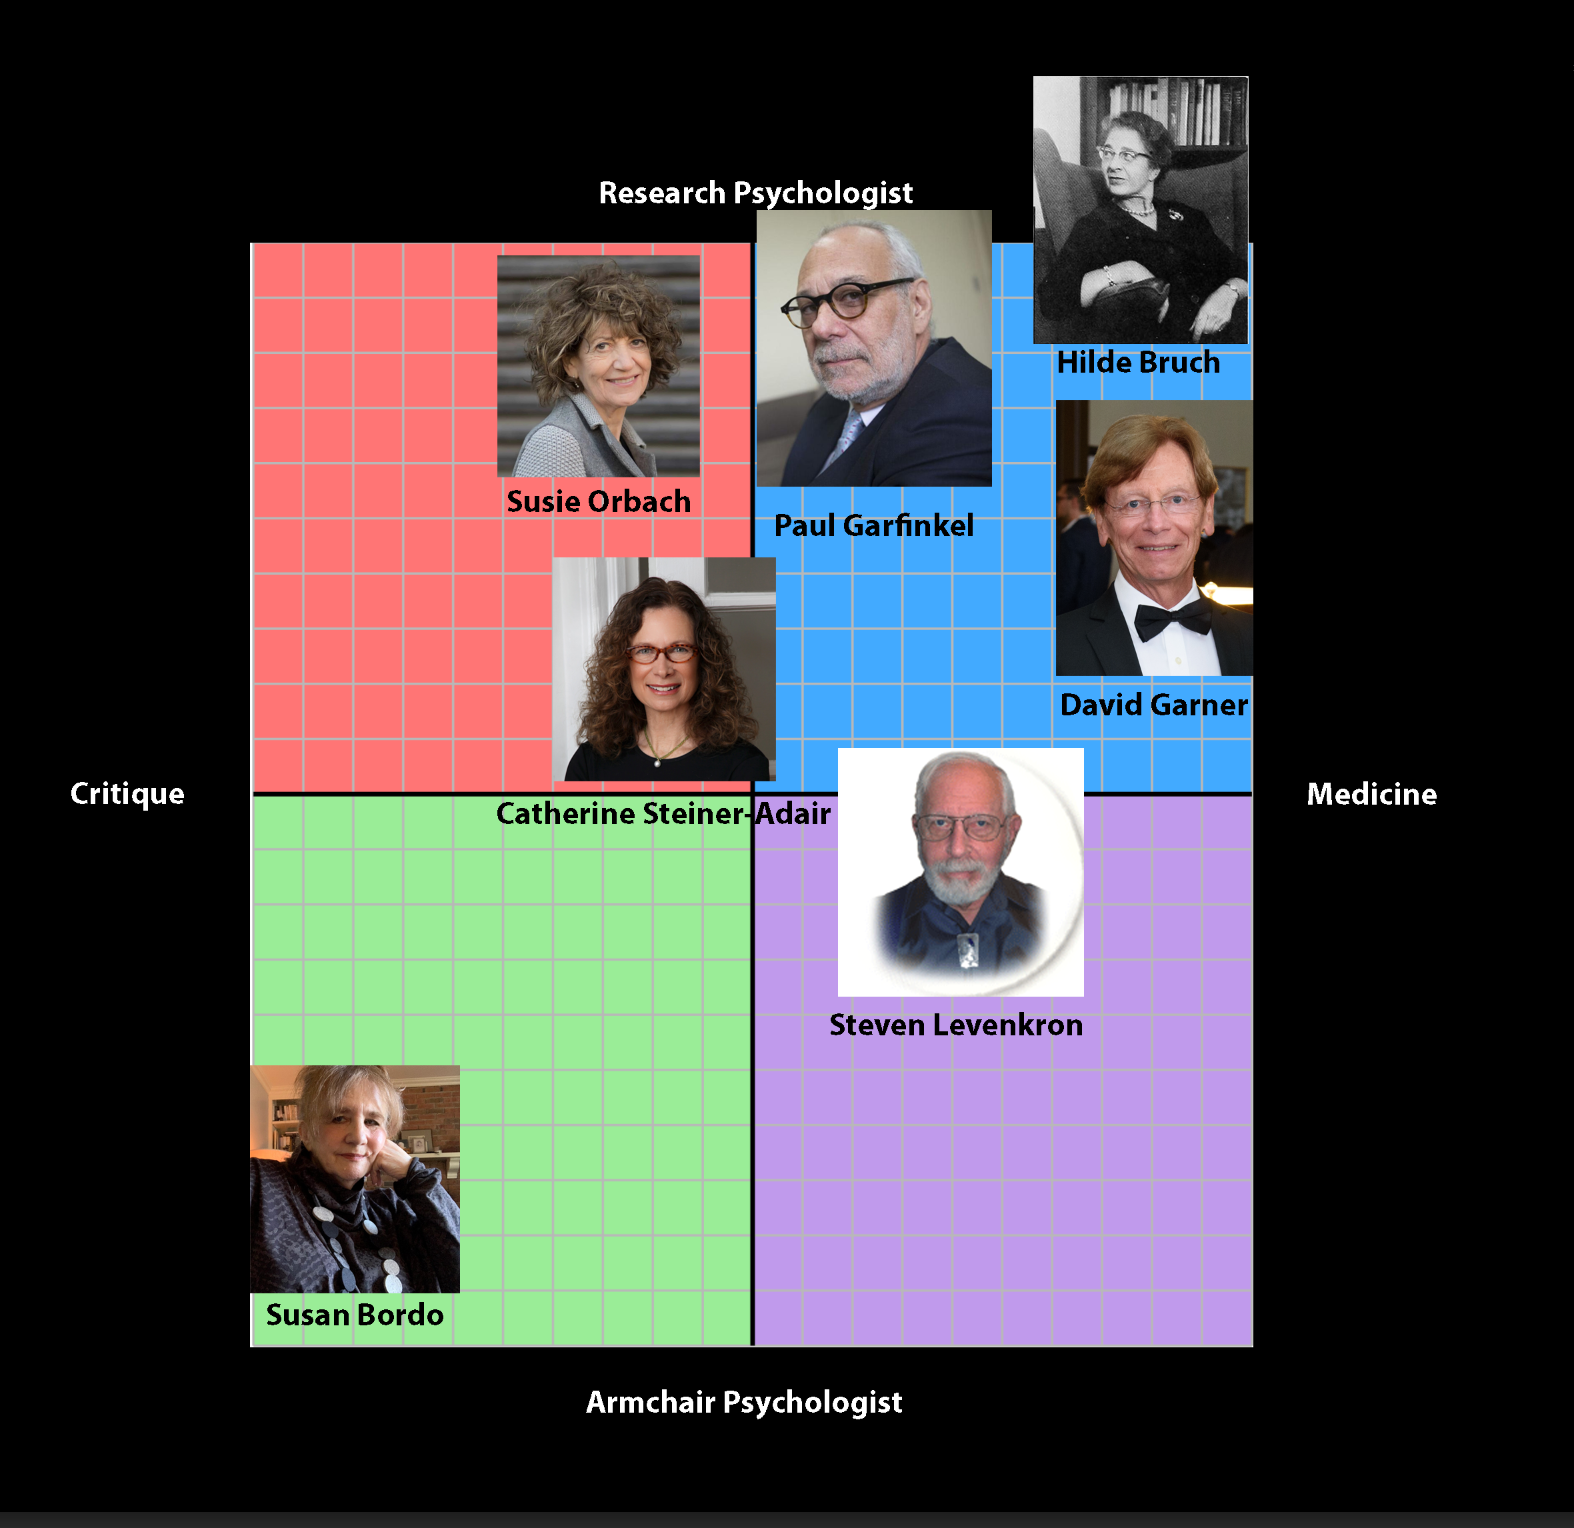
\includegraphics[width=\textwidth]{alignment chart print 1.png}

    \begin{itemize}
        \item Catherine Steiner-Adair, for example, describes herself as a ``clinical psychologist, consultant, author, speaker'' -- her early work as cited by Bordo has the trappings of psychological research but falls more, in my opinion, under the umbrella of social critique. She is credentialed as a Doctor of Education, which is usually associated with practical work in education, and is separate from a PhD in Education, which tends to be more research-oriented.

        \item David Garner and Paul Garfinkel, at least in the era we're talking about, were both psychological researchers. Garner was the head of research at Toronto General Hospital, while Paul Garfinkel is a medical doctor and serves on the psychiatry faculty at the University of Toronto. 
    \end{itemize}
    There are two other people we haven't discussed yet who appear frequently in the discourse of the time:
    \begin{itemize}
        \item Bordo favorably mentions psycholgist and feminist writer Susie Orbach, who we'll talk about in a minute. Orbach was a psychologist and practicing psychotherapist in England, but is most well-known for her social criticism.
        \item Bordo criticizes Steven Levenkron, a psychotherapist and alleged (by me) sex pervert in New York, who wrote not only several clinical texts about eating disorders, but also some highly suspect, remarkably fetishistic novels about young girls with eating disorders, apparently inspired by his own patients. 
    \end{itemize}

    What sets Susan Bordo apart from all these people, of whom she has varyingly friendly and adversarial opinions, is that she is not a medical practitioner -- she certainly does not have patients, and her work is generally uninterested in providing advice or improvements to people's lives. She is also not a psychology researcher -- her work is equally unconcerned with scientific fact as it is with the practical reality of individual lives. So, what does she have to contribute? 

    Personally, I find her critique of what she calls the ``biological argument'' both accurate and necessary. She says that biological features and predispositions are not good approaches to assessing the overarching cause of an eating disorder, which has become the consensus among experts. I also find that, were one to have a philosophical or literary characterization of eating disorders, her idea that the disorders represent one's embodying of certain internal contradictions is as good as any. However, ironically, in her rush to describe a monolithic cultural force responsible for such disorders, Bordo forgets \textit{people}. The contradictions in play for her are always societal and generalized, sometimes coming into contact with an individual's body but never outside the realm of the abstract. Besides the biological, Bordo discards anything that could also be on an afflicted person's mind: familial relationships, sexual abuse, gender dysphoria, depression -- the family of ``the anorexic'' in abstract is abstracted further into stereotypes of ``the mother'' and ``the father'' while sexual abuse is replaced with cultural norms of desirability, depression is always the result of patriarchal oppression, and any sort of unfeminine gender expression is itself a life-threatening disorder.~\footnote{See ``the mother's actual lack of position and authority outside the domestic arena,'' \Cite[207]{Bordo03}; how ``anorexia will erupt, typically, in the course of what begins as a fairly moderate diet regime, undertaken because someone, often the father, has made a casual critical remark,'' \Cite[178]{Bordo03}. Both of these are taken to simply be truisms.}

    \subsection*{Susan Bordo thinks that 90s TV talk shows were pushing trans ideology}

    This strange relationship Bordo has with people with eating disorders informs and is informed by the equally strange views she has about gender. Alongside Steiner-Adair's work, Bordo discusses the views of feminist writer and psychologist Susie Orbach. She defends Orbach against some highly problematic criticism, including from the same David Garner, who characterized Orbach as inflicting ``guilt'' on mothers ``for `choosing traditional values.''' However, interestingly, Bordo's defense against criticism from Steven Levenkron (psychotherapist and author of the remarkably fetishistic anorexia novel \textit{The Best Little Girl in the World}) that Orbach ``failed to appreciate adequately'' the suffering of ``the anorectic herself'' was only to suggest that Levenkron was refusing to engage with Orbach's political ideas and deflecting by questioning her empathy and concern ``with actual women's lives.'' This is all likely very true; however, like Steiner-Adair's purported causal relationship between eating disorders and cultural unawareness, Bordo's concern does not actually appear to lie with the suffering of anorexic people or of women, nor does she trust them to understand their own disorders. If this seems too harsh, we should at least take it as a reminder that we are discussing real individuals' deeply personal and potentially dangerous conditions, subjects about which we should feel obligated to talk with at least a little care and delicacy. Orbach, too, questions the doctrine that anorexia is a pathological condition, instead arguing that it constitutes ``one extreme on a continuum on which all women today find themselves.'' This, I think helps to explain Bordo's willingness to represent science as she does -- if all women are, universally, at least miming anorexia, studies like Steiner-Adair's don't need to justify that their results hold across the whole population, for women in general; they would only need to give a single example of any association between mass culture and an eating disorder, however isolated. Universality, for her, is a given.~\autocite[47]{Bordo03}

    So, by tacitly presupposing that eating disorders are cisgender women's diseases, what does Bordo miss? Well, a lot. To see this, we're going to take a look at the way eating disorders affect trans people. A 2019 meta-analysis estimated the twelve-month prevalence of all eating disorders to be 2.2\% for women -- that is, in any twelve-month timespan, 2.2\% of women across America, Europe, and Asia are likely to meet a disorder's diagnostic criteria.~\autocite[1406]{Galmiche19} This would include anorexia nervosa, bulimia nervosa, and binge eating disorder. However, a study of 3,371 trans people, based on the results of two surveys conducted between 2017 and 2019, screened 35.04\% of participants as potentially having either anorexia or bulimia, and recorded that 10.46\% of all participants had a previous clinical diagnosis.~\autocite[449]{Romano21} The prevalence within each designated group (trans man, trans woman, or genderqueer/nonbinary) was roughly the same.

    One applying Bordo's theory might be tempted to say that this is an example of recent proliferation of disordered eating, like she says about men and non-white racial groups. However, this would be nothing more than an assumption. Since (for what I hope are obvious reasons) none of the research available to Bordo in the 1990s reported any data for transgender people, there's no reason to assume that the high prevalence of disorders for them is anything new. Similarly, if one were to suggest (parallel to Bordo's claim that anorexia in racial minorities emerged due to their newfound opportunities after the American Civil Rights era) that this is actually the result of more mainstream acceptance of trans people recently, it would likewise be a guess and would greatly overstate the degree to which hegemonic culture is willing to accept transness. 

    Now, a more direct response might be to take this as the purest example of her cultural theory, making trans people into a literal embodiment of the same masculine-versus-feminine tension, the ```androgynous' ideal that ultimately exposes its internal contradiction and becomes a war that tears the subject in two'' that allegedly causes eating disorders in cis women.~\autocite[174]{Bordo03} This is problematic for many reasons, and it shouldn't go without saying that viewing trans people as being torn apart by the irreconcilable battle between masculinity and femininity is deeply transphobic, not to mention that it ignores the many genderqueer people who identify as neither men nor women. More immediately, though, it would ignore the opinions of actual trans people with eating disorders, some of whom were interviewed as part of a 2022 report. While, as we've learned, it would be careless to take these responses as representative of the entire worldwide population of trans people, one still might imagine that we could learn something from listening. 

    First, while participants did identify gender dysphoria as a motivation towards eating disorders, it was a motivation equally significant for trans women, trans men, and nonbinary people. One trans woman associated it with ``American cultural ideals about what a pretty woman looks like,'' which would appear to support Bordo's explanation, but one trans man associated anorexia with ``hating [his] body because it was too feminine'' and ``getting rid of curves.'' If we were to accept Bordo's model, an anorexic body would have to be an ideal both for men and for women, which she certainly does not believe. Similarly, several people associated their eating disorders with a conscious desire to slow down puberty.~\autocite[426]{Cusak22}
    
    Second, many respondents, again from a variety of gender identities, ``described cognitive (e.g., feeling the need to control their body), affective (e.g., shame, disgust,
    guilt), and behavioral (e.g., avoidance and self-punishment) components that reflect strategies to manage negative emotions associated with one's gender identity and body.'' While Bordo frequently mentions the desire for control in relation to cis women, she only mentions shame as something that is culturally-inflicted and always in relation to appearance or weight, and it would be a mistake to assume that feelings of guilt associated with transness are only the result of pervasive cultural transphobia. Bordo does not consider self-punishment as a factor, excepting self-punishment for lapses in a diet, but respondents did not always make that connection. Instead, ``punishment for some participants was described as outside of themselves, onto their body, whereas others spoke of punishment directly related to who they are as persons.''~\autocite[427. It would be deeply misguided to view this as the same sort of shame that Bordo suggests all women are taught to feel for their femininity. Not only is that cultural shame not comparable to the societal disgust often shown towards trans people, sometimes people, without external indoctrination, might just not like themselves very much.]{Cusak22} Incidentally, more general research has found ``a significant association between continuous combined measures of discrimination and combined ED psychopathology,'' which could indicate a cause for eating disorders among discriminated-against peoples entirely unrelated to beauty.~\autocite[410]{Mason21}

    Now, to be fair, the most common issue identified by respondents was gender expression and associated ``external appearance standards, such as masculinity, femininity, and androgyny.'' But, are these appearance standards the same cultural ones that Bordo presumes? One nonbinary participant said they ``have an attractive AFAB body, athletic and relatively thin, and [have] a hard time reconciling the desire to be conventionally attractive with the desire to be seen as a nonbinary person'' and that ``when [they] first wake up and [their] stomach is flatter [they] feel more masculine.'' For this person, the idea of being a conventionally attractive woman is actually in opposition to their desire to restrict. On the other hand, one trans woman said that she feels obligated ``to follow feminine beauty standards more strictly than others otherwise [her] gender will be called into question,'' associating restrictive behavior with a feminine appearance. One agender participant said that, to them, ``skeletons always seemed androgynous.'' \autocite[427-428]{Cusak22}

    So, we have a collection of people, of various genders, associating thinness and the act of denying oneself food with their own gender identities, regardless of what those identities are. This differs from Bordo's understanding of masculine eating disorders, which she sees as aspiration towards a conventionally-attractive, male-coded muscular body, and exposes the nuance lacking in her understanding of eating disorders outside the gender binary. Respondents of all gender identities associated with their gender practices which Bordo believes, to this day, are idiosyncratically feminine. 

    You might object to my insistence that Bordo's speculated androgyny in anorexia is rooted in flawed abstraction rather than lived experience when she herself says that this ``battle between male and female sides of the self'' is how those with the disorder characterize it, referring us to the chapter ``Anorexia Nervosa.''~\autocite[174]{Bordo03} This section concerns several narratives written by anorexic and bulimic women, potentially connecting their experiences to her cultural theory. While not quite the framing of the ``many anorectics'' she suggests, it was at least the theory given by Aimee Liu, who suggests that her own anorexia was a ``plotted'' escape from her body, ``the flesh that teased them--'' that is, sexually abusive men -- and that the route of escape was ``to become androgynous.''~\autocite[As it happens, Liu's memoir was reprinted in 2013 with an additional preface, in which she reflects on her conceptions as a twenty-five-year-old: ``Unfortunately, our society's emphasis on appearance has intensified in the intervening decades, and the academic and emotional pressures on adolescents have only escalated. At the same time, scientific research has shown that eating disorders are much more complex conditions than I realized when I was writing about my own experience. Genes play a large role in determining who is vulnerable to anorexia and bulimia, and who is not. So do brain chemistry and biological temperament -- personality.'' In a simple and, I felt, touching way, she ends the preface with: ``For me and virtually every other person I've ever met who's suffered from an eating disorder, that problem involves identity. Who am I in the world? Why don't I know who I am? Why am I forced to be someone different than who I am? Why do I feel so wrong? Why can't others see that I feel empty inside?'']{Liu13} Liu's phrasing stands out among Bordo's other examples, who, rather than androgyny, say they seek ``absolute purity, hyperintellectuality, and transcendence of the flesh;'' or ``energy, discipline, my own power;'' or ``pure concentration, energy, and spirit.''~\autocite[150]{Bordo03} This juxtaposition only makes sense, though, if we accept first that by ``androgyny'' she really means unfemininity, and second that each of those descriptors is inherently unfeminine, assuming the very thing she wants to prove: that anorexia is necessarily a pursuit of that unfemininity. 

    More prominently, Bordo pulls this application of a split masculine/feminine self from Hilde Bruch, who recounts that anorexic patients often characterize their food-averse inner monologue as an ``other self'' who is apparently always male.~\autocite[155]{Bordo03} While the complicated and problematic implications of Bruch's \citetitle{Bruch01}, especially with regard to gender, are outside the scope of my study, she sees the masculine coding of this inner voice as, while perhaps associated with gender confusion, stemming more from childhood perfectionism.~\autocite[55]{Bruch01} This is broadly in-line with the way Bordo supposes ``perfectionism'' to be a trait usually associated with masculinity. Incidentally, Bruch's text, which recounts her interactions with several patients receiving treatment for eating disorders, features several male subjects whose behavior is not differentiated from the other, female subjects -- but Bordo neglects to mention them. This is also the moment where Bordo differentiates, by philosophy rather than practice, anorexia and bulimia: unlike those with anorexia, ``in the binge-and-vomit cycle,'' a bulimic person's ``hungering female self refuses to be annihilated'' by the male self. She claims that bulimia is not constituted by ``the rejection of femininity,'' which is why women with bulimia apparently ``tend to strive for a more `female-'looking body as well.''~\autocite[324][(what the fuck?)]{Bordo03} We'll come back to this.

    \subsection*{Is it gay to be marginalized by the healthcare system?}

    In order for anorexia and bulimia to be so inseparable from troubled femininity, Bordo must then show that men and women express the disorders via different behaviors and with different goals. In ``Hunger as Ideology,'' Bordo tries to demonstrate a determinative link between gendered images in advertising concerning food and the ostensibly gendered nature of anorexia and bulimia. She treats us to another scientific citation, asserting that there is ``an extremely interesting fact about male bulimics: they rarely binge alone.''~\autocite[128]{Bordo03} There are indeed several extremely interesting things about the study she believes contains this statistic, ``Bulimia in Males: A Matched Comparison with Females'' by John Schneider and W. Stewart Agras. First, over half of the men tested did not identify as heterosexual. This is not a sidenote -- Schneider and Agras explicitly claim that ``male heterosexuals appear to be protected against the development of bulimia.'' The exact proportion of non-heterosexual male respondents was in fact eight out of fifteen, as -- and by now this may be unsurprising -- only fifteen men participated in Schneider and Agras's study, and only thirty subjects did in total. More shocking is that Bordo's claim that male bulimics ``rarely binge alone'' is in fact not present in Schneider and Agras's publication. They do relay that ``males reported being less likely to eat and binge alone'' while women ``reported eating less at a meal and [preferred] to binge in private,'' which is quite far from Bordo's exaggeration. But this is not just stylish hyperbole -- she needs to overplay any potentially-gendered difference she can, because anything less than a perfectly clear-cut divide between male and female behaviors would immediately make her gendering of disordered behavior highly suspect.
    
    Interestingly, while the male participants in the study volunteered information about their respective eating disorders in response to newspaper advertisements, the female participants were sampled from preexisting patients at the Stanford Eating Disorders Clinic. Although some comparisons can be made with this method, they would not be comparisons between the greater populations of men and women with eating disorders. Again, individuals who are diagnosed and undergoing treatment for a disorder are not directly comparable to self-identified sufferers who respond to an advertisement. Now, despite the small sample and statistical inapplicability of Schneider and Agras's work, I don't mean to say that its results are incorrect. The variance they found in their sample may very well generalize to a larger population, but the only thing we can conclude from this study alone is that perhaps a larger, more representative study is warranted. Schneider and Agras make exactly this sort of assessment in their conclusion, which raises a somewhat obvious concern about researching sex differences in eating disorders that Bordo really should have considered:
    \begin{adjustwidth}{40pt}{0pt}
        Overall, bulimia in males may be underdiagnosed because the disorder has typically been described as occurring in adolescent women. Given this focus, males with bulimia may be hesitant or embarrassed to discuss the disorder, or may deny the problem altogether (as initially was characteristic of women with bulimia). The males in this study did express embarrassment about attending the clinic for bulimia, were unstable in keeping appointments, and tended to drop out of treatment. Health care professionals familiar with female bulimics may not be considering bulimia as a possible diagnosis in males because the presenting symptom duster, etiology, and personality characteristics and weight history are somewhat different than with women. It may well be that the small number of men identifying themselves as bulimic underrepresents the true prevalence of males with this disorder.~\autocite[238, 241]{Schneider87}
    \end{adjustwidth}
    It's also interesting that Bordo doesn't think it's important that this study was of mostly homosexual and bisexual men, considering that she associates the behavior of these men with imagery in advertisements that are expressly heterosexual. In fact, her only mention of queer sexualities at all was to say, without basis, that ``lesbian cultures in the United States continued to be accepting \dots of fleshy, spaceclaiming female bodies'' in the early 1970s, but in later decades this was ``no longer as acceptable as it once was in lesbian communities.''~\autocite[103]{Bordo03} True or not, this is an afterthought that suggests she views lesbian beauty standards as essentially interchangeable with heterosexual stereotypes of femininity and that this change over time is due in large part to media images. The second point is especially bizarre because she argues for an expressly heterosexualized interpretation of those media images.

    So, Bordo's disinterest in the medical model is problematic, because it justifies a profound disinterest in factual accuracy, but it's also depressing, because ``Hunger as Ideology'' depends on an ideology of medicine that she fails to see. In broad strokes, her theory could be convincing: advertisements tend to praise women for not eating and for being thin while simultaneously depicting men of various sizes eating freely, so audiences are conditioned to associate thinness with femininity and to dissociate masculinity from ``the body''. We can object to the assumption that a viewer would necessarily (or even usually) identify themselves with someone of the same gender in an advertisement (especially since much of this identification depends on a presumed heterosexuality), but it does seem plausible that such an identification might occur particularly with regard to thinness. The problem is that Bordo takes this identificatory relation for granted, which causes her to neglect the more interesting question of precisely how it might occur. 

    She has already decided that there is no essential difference between anorexia and womanhood, so what use would she have anything that claimed to screen for something that must already be there? She is equally uninterested in causes for eating disorders in males because their disorders cannot be adequately understood in this way -- so she reclassifies male eating disorders as having different cultural causes, stating, without a source, that disordered males ``are almost always models, wrestlers, dancers, and others whose professions demand a rigid regime of weight control.''~\autocite[53]{Bordo03} According to her, men with eating disorders are fewer relative to women because men's disorders result from rare professional or personal demands rather than the contradictory cultural demands placed on, I guess, all women. This would suggest that, while psychometric data designed to differentiate anorexic women from nondisordered women is in fact only reporting the severity of the condition all women have, the same data can be, for some reason, trusted to show that men with eating disorders are merely outliers, even while statistically shown to be unreliable on male samples. 
    
    \subsection*{Why it's important to read books relevant to your field of study}

    We start from a place of agreement -- the claimed implications aside, Bordo convincingly shows that it was rare in 1993 to see in advertisements women eating. The aberrant behavior, a woman eating, is made pathological but this motion is not unmotivated -- on the other hand, a woman not eating would be necessarily pathological because Bordo invariably sees her as a spectral implication of an eating disorder. The result is that food itself is pathologized -- by the inventions of obesity, BMI, and the calorie. But these are regulations of a medical ideology, merely some among a myriad of other medical regulations. If we take anorexia to be a medical invention (i.e. a thematization of specific acts rather than an irreducible biological condition), then how could its relative prevalence in women be determined by the regulatory apparatus of medicine? How might its diagnostic criteria or social stigma or the biases of doctors lead to its invention as a women's disease, and how might that help to enforce a heterosexist dichotomy in medicine? What motivates the acts it thematizes or, put another way, what other behaviors or conditions does the medical system regulate through eating disorders by proxy? How could we even identify the individual practices of medical self-regulation characteristic of eating disorders? Bordo doesn't challenge the medical institution's construction of eating disorders -- only appropriates it when useful and ignores it when not and, in doing so, reifies its sexist ideology and obscures the very bodies in which she is interested behind an opaque ``The Body,'' fundamentally unable to explain why hunger supposedly signifies femininity.

    Because Bordo is unconcerned with the specific physical self-regulatory practices associated with eating disorders, it can be difficult to decode exactly what she believes those practices to be, particularly for anorexia as it lacks the ostensibly identifiable, singular practices of bulimia and binge eating disorder. However, Bordo regularly indicates that the central motivation of people with anorexia is to appear thin, usually for beauty-related reasons. Now, entertaining her premise that this is to some degree a feminine universal, is this consistent with the disorder as understood by others? In the 1980s, the diagnostic criteria for anorexia nervosa consisted of five features:
    \begin{adjustwidth}{40pt}{0pt}
        \begin{flushleft}
        A. Intense fear of becoming obese, which does not diminish as weight loss progresses.

        B. Disturbance of body image, e.g. claiming to ``feel fat'' even when emaciated.

        C. Weight loss of at least 25\% of original body weight \dots.

        D. Refusal to maintain body weight over a minimal normal weight for age and height.

        E. No known physical illness that would account for the weight loss.~\autocite[68--69]{DSMIII}
        \end{flushleft}
    \end{adjustwidth}
    Although the phrasings of the latter three would be interesting to someone more critical than Bordo of the assumptions underlying medical ideology, they are relatively unsurprising for the era. The fear in Criterion A could agree with Bordo's model, where it would be the self-centering of an extrinsic fear of being perceived as lesser in a society that views being fat as a defect (medically and morally) -- but one would then expect that fear to become less prescient for thinner people. Bordo's model attempts to explain this by interpreting the warped body image of Criterion B as one's extreme, total internalization of that social compulsion. This condescension is (as Steiner-Adair demonstrates) tempting -- but is ultimately incorrect. Even though the literature at the time notes that ``most individuals with this disorder steadfastly deny the illness and are uninterested in, even resistant to, therapy,'' it does not suggest that they are unaware of it. With the perceived consequences and loss of control in mind of admitting a disorder (not to mention the medical subjection that would follow such an admission), unawareness would seem extraordinary. More pressingly, this explanation would unavoidably conflate ``feeling fat'' with ``appearing fat,'' presupposing the centrality of outer perception that Bordo seeks to prove in the first place.

    I don't mean to suggest that the DSM-III is a reliable description of any eating disorder, or that any version of the DSM exists to do anything but legitimize the decisions of the health insurance industry. Still, the diagnostic criteria have been revised substantially since then: there are now three features, with the amount of proportional weight loss in the older Criterion C made more nuanced and the remaining condensed to:
    \begin{adjustwidth}{40pt}{0pt}
        \begin{flushleft}
        B. Intense fear of gaining weight or of becoming fat, or persistent behavior that interferes with weight gain, even though at a significantly low weight. 

        C. Disturbance in the way in which one's body weight or shape is experienced, undue influence of body weight or shape on self-evaluation, or persistent lack of recognition of the seriousness of the current low body weight.~\autocite[338--342. The revised criteria offer some other cautions to the more philosophical analyses of anorexia. For example, rather than results of confounded femininity, depressive symptoms such as mood issues and lowered interest in sex are ``also observed in individuals without anorexia nervosa who are significantly undernourished'' and ``may be secondary to the physiological sequelae of semi-starvation.'' This should be of particular interest to Bordo, who believes that low sexual activity in anorexic people stems from attempts to reject femininity.]{DSMV}
        \end{flushleft}
    \end{adjustwidth}
    Although Criterion B might appear essentially the same as the older Criterion A, the ``or'' is not an accident. The manual remarks that, in fact, fear of gaining weight is, while common, not the only justification given for one's restricted food intake, and appears less in populations in Asia as well as in Latino populations in the United States. Now, we don't really need to speculate on the role ethnicity plays here -- the critical point is that concern with weight or fatness is actually not an essential feature of anorexia as it's understood more currently.

    Bordo's description of restricted eating motivated primarily by weight and secondarily (inextricably) by appearance seem more consistent with dieting than with anorexia or bulimia. Both her habit of hiding personal experience behind overgeneral abstraction and her odd belief that anorexia is essentially the inevitable consequence of womanhood are somewhat explained once we realize that Bordo doesn't really understand the difference between the two. Regardless of the underlying cultural reason Bordo imagines, in the individual anorexia is the natural and essential result of wanting to be beautiful. 

    On some level, she seems kind of aware that the conflation is problematic. At least by 2009, she thought to include the caveat that ``it's incorrect \dots to imagine that this is simply about beauty'' in an article commenting on the apparently-broadening diversity among people with eating disorders. She mentions finding it ``fascinating and illuminating'' to hear that some Nigerian women were ``dieting'' in what one described as a rebellion against a traditional, highly patriarchal marital system, and that this certainly predated a thinner Nigerian model, Agbani Darego, winning a televised beauty pageant, which Bordo had previously assumed was the media moment responsible for the women's behavior. Unfortunately, this moment of illumination was fleeting. In still describing Darego as providing ``an alternate cultural paradigm to aspire to,'' Bordo betrays that she still sees aspirations of beauty to be more important than the more internal concerns of fasting Nigerian women who ``had been sexually abused, or witnessed their own mothers being treated badly.'' Incidentally, it also perfectly exemplifies her mistrust of African women, who apparently would never have associated thinness or restriction with resistance to misogynistic oppression unless instructed how by ``western body ideals.''~\autocite[270-271]{Bordo09}

    This makes it especially comical when Bordo claims that, in writing \textit{Unbearable Weight}, she was ``virtually alone in viewing eating and body image problems as belonging to anyone except privileged, heterosexual white girls.''~\autocite[266]{Bordo09} Now, this isn't true -- obviously.~\autocites[Certainly in the medical sphere -- aside from Schneider and Agras above, see][]{Yager87}[see][-- but also in widespread discourse]{StriegelMoore90}[see][204, for a surprisingly nuanced discussion of body image in relation to social class]{Bourdieu84}[see][for a popular magazine article comparing various body image perceptions between men and women as well as between age groups -- and even in fiction]{Cash86}[see][a novel about, in part, a Zimbabwean girl suffering from bulimia and the relationship between her disorder and colonialism which is far more complex than viewing it as an internalized ``western body ideal.'' All of these predate \textit{Unbearable Weight} by several years.]{Dangarembga88} Even if she spent anywhere near the amount of time on non-white or non-heterosexual or poorer or non-female people that she did on that one particular group, and even if she had bothered to question the validity of clinical data that she herself cites, she would still have been making the case that eating disorders \textit{originated} in privileged, heterosexual white girls. Others are permitted to watch privileged, heterosexual white girls and learn from their example, even emulate their behavior, but not to claim this alleged ideal image for themselves. Eating and body image problems are still the property of, if not privileged, heterosexual white girls, then, according to Bordo, of their culture. Every time Bordo tries to mention eating disorders in more diverse demographics rings hollow -- she is occasionally aware of contradictory statistics but she doesn't want to believe that they really refer back to the same disorders. 

    I think this encapsulates the inadequacy of ``body studies'' as a discipline. The claims to specificity, to lived experiences, potentially convincing to some, will always be transparent to anyone not included in the myth that is The (universal) Body. But the violence of exclusion and the violence of inclusion -- the violences of bodily appropriation for some disconnected, impersonal theory -- are comorbid. \textit{Unbearable Weight} commits both. Since its publication, \textit{Unbearable Weight} has been criticized for its failure to adequately or appropriately consider eating disorders in marginal populations, but, as we've just seen, she not only rejects this criticism but believes her book to be the most inclusive representation of them possible at the time. She mentions, finally, the skewed population statistics that led to this bias in ``scientific and social-scientific explanations'' but fails to consider how this bias demonstrably affected her own work. She asserts that ``the medical literature often conflated class and race'' when they concluded that since ``poor people didn't get eating disorders \dots how could black people?''~\autocite[266-267]{Bordo09} Her problem here is with the racist reasoning but, significantly, she makes the very same assumption in \textit{Unbearable Weight}, suggesting that anorexia ``depends on certain material preconditions which economically struggling women lack,'' or at least that such a divide did exist in the past.~\autocite[62]{Bordo03} 

    \subsection*{The system needs bodies}

    So, 1993 was a long time ago and, since we're discussing an academic world both near enough for some to remember yet far enough that I can't, let's briefly check in to see where our main characters are today. 

    Catherine Steiner-Adair appears to be working in corporate consulting -- her website has been recently updated to describe her work as ``ensuring that today's students - our children - have not just the technological tools they need as they inherit the AI future, but \dots DEI competencies they need to survive,'' etc. I wish her the best of luck revising her bio when these buzzwords fall out of fashion. Steven Levenkron appearts to be still practicing as a psychotherapist, unfortunately. His last book has two reviews on Amazon, for an average score of $1.6$ stars, so I wish him better luck with the next one. David Garner was suspended from the College of Psychologists of Ontario for ``sexual impropriety'' in 1988, three years after he began a sexual relationship with an eighteen-year-old patient he was supposed to be treating for anorexia.~\footfullcite{Ontario88} Paul Garfinkel wrote an editorial highly critical of Garner, who went on to have his license to practice in Ontario revoked permanently in 1989 after another sexual abuse victim came forward. At some point, Garner opened an eating disorder treatment center in Sylvania, Ohio, from which he resigned in 2003 after having an affair with an employee and being charged with fifteen ethics violations by the Ohio State Board of Psychology.~\footfullcite{Blade03} I hope he rots in hell. Susan Bordo herself has been writing your standard, run-of-the-mill, convictionless, pro-Democratic-Party political posts on Substack all year, first somewhat hilariously shilling for Joe Biden --
    
\includegraphics[width=\textwidth]{bordotweet1.png}

    while also talking extensively about how war criminal Hillary Clinton was similarly maligned -- and then immediately pivoting to equally shameless shilling for Kamala Harris. I'm not going to get in to her political beliefs, but I think they are, you know, bad.~\footnote{\url{https://susanbordo.substack.com/p/bernie-sanders-put-that-wagging-finger}}

    From reading \textit{Unbearable Weight} for the first time, I recall feelings of suspicion, on account of the essentialist gender politics and Bordo's tenuous relationship with scientific data, but deeper than that, I recall a feeling of offense -- what gives Susan Bordo the right to speak so declaratively, regressively, and incorrectly about actual bodies? In the brief personal situating she performs, she identifies herself as explicitly not anorexic, saying that ``[her] own disordered relations with food had never reached the point of anorexia or bulimia'' and that she would ``include [herself] among compulsive eaters'' who are ``left out of the `anorexic paradigm.'''~\autocite[268]{Bordo09} On one hand, she insists that her own dieting for appearance-related reasons is archetypal for all women and (necessarily, in her opinion) all anorexics, either ignoring contrary experiences or rewriting them. On the other, she cannot entertain the idea of hunger that's self-motivating -- that doesn't hurt. 
    
    There's this excuse Bordo uses time and time again in asserting the universality of her reactionary ideology -- that \textit{she} doesn't believe that women are corporeal while men are intellectual, passive while men are active, dependent while men are autonomous -- but that ``the culture'' does believe it. This is so vast an overgeneralization that it belies not just the small, narrow view that Bordo has of mass culture, but also the degree to which she is unwilling to interrogate her own harmful attitudes. She makes my body her own, in the guise of making it ``the culture's.'' 
    
    In what could be charitably called a moment of vulnerability, Bordo talks in a more recent article about how ```the culture' includes parents, too,'' and that her own complexes around food and appearance are likely to have an influence on her daughter, Cassie. But, making this relationship entirely a cultural one, she absolves herself of responsibility for the bodily harm she may commit. Now, being as fair as I might possibly be, this is forgivable -- we are not always in control of who sees us engage in disordered behaviors, and even the most conscious parent can't be expected to perpetually hide how food affects them, especially in a cultural climate so equally conscious of this. Unfortunately, Bordo says about Cassie that ``it's hard to imagine her ever becoming ashamed of her body,'' but I can imagine it. I could imagine it the moment Cassie's dear mother decided she had ``a tummy we would all \textit{die} to have'' before then deciding that it was okay to publish those words in a book that people would read.~\autocite[273-274 (original emphasis)]{Bordo09}

    This is at once the conceit and the failure of body studies. In her research, Seaber observes the phenomenon of eating disorder life stories that are, as literature, full of cautions and warnings and tragedies and are yet taken as tips, ideals, disidentificatory inspiration by people with those disorders. She locates an undercurrent of thinspiration throughout the genre, beginning with Levenkron's \textit{The Best Little Girl in the World} and the sexual component of its visual fixation with anorexia that ``dwells specifically on what the bodies look like and on Kessa's obsessive, repetitive, haptic interactions with her own body -- in ways that read as sexually voyeuristic rather than more generally or disinterestedly descriptive of physical appearance.''~\autocite[60]{Seaber21} Subsequent eating disorder narratives, with their potentially conflicted authors, sometimes engage in tactical misreading of preceding narratives, in what Seaber calls ``disordered reading--'' a practice wherein ``readers privilege their interpretation of certain textual events over any number of others that may contradict it.''~\autocite[490]{Seaber17} Her main example is Marya Hornbacher's \textit{Wasted}, in which the author identifies the moment where she, as a child, takes disordered inspiration from Levenkron's novel, and which would go on to serve the same purpose for some of its own readers. But what explains Levenkron? Well, he's an alleged (by me) sex pervert, but what I mean is: what explains body studies' parallel tradition of misreading nearly everything regarding the lived experiences they purport to represent? 

    Hadley Freeman's \textit{Good Girls} is but one of many of these stories, a personal narrative infected by disordered reading, by self-serving falsehoods and selective memories. What sets it apart is that -- and I apologize for the suspense -- Hadley Freeman is a transphobic columnist, formerly employed by \textit{The Guardian} until quitting in protest when the magazine refused to run her interviews with prominent transphobes,~\footfullcite{Telegraph22} following public backlash for dismissing suicide risks among trans kids. Specifically, she thinks that any vocal suicidal ideation among trans kids are just empty threats, manipulation ``if their parents didn't help them get sex change hormone and surgery.''~\footnote{\fullcite{Vice20}; \fullcite{PinkNews23}} 
    
    So, when Freeman says that ``just as doctors have long suggested a potential overlap between anorexia and autism, some are now noting a similar one between anorexia and gender dysphoria,'' (citing two studies, neither of which actually make that claim), or that ``gender dysphoria differs from anorexia in one important aspect: anorexia is deemed, rightly, to be an illness that requires treatment'' while ``gender dysphoria is not and is often defined as an expression of the person's authentic self,'' or when she quotes Dr. Melissa Midgen (who is not a medical doctor)\footnote{and whose Twitter presence is mostly agreeing with Hadley Freeman and holocaust denier J. K. Rowling, incidentally.} saying that gender dysphoria ``could be the new anorexia,'' she isn't just some neutral observer.~\autocite[idk which page -- I got the ebook]{Freeman23} She makes this (hilariously false) comparison for political reasons, because she believes that trans people are aberrations, diseased people who need to be cured. 

    More fundamentally, though, Freeman, like Bordo with thin bodies or like Levenkron with his patients' bodies or especially like Garner with his patients' bodies, sees people's bodies as hers to appropriate. In her introduction, Bordo describes her goal with \textit{Unbearable Weight} as ``consciousness-raising,'' at least in theory explaining the nature of eating disorders while simultaneously admitting the possibility of this ``servicing an oppressive system.''~\autocite[31]{Bordo03} But her conception of this oppressive system is one that depends totally on false dichotomies, particularly of gender, and by writing without questioning these dualities she can only reinforce them. She scornfully dismisses this criticism as one that ``depends upon so abstract, disembodied, and ahistorical a conception of how cultural change occurs as to be worthy of inclusion in the most sterile philosophy text.'' Even if challenging dualities was as boring as she appears to find it, I find it strange to say that ``culture shifts \dots through real, historical changes in relations of power'' but to exclude discourse -- her discourse -- from having any sort of influence on culture. Her second excuse is equally pathetic -- that she would love to challenge ``hierarchical oppositions (male/female, mind/body, active/passive)'' but that ``it is not so easy to `go beyond dualism.'''~\autocite[15]{Bordo03} To this, one could say that maybe she should have tried harder, because if these dualities are so unchangeable, the only purpose this work could serve, with its abject failure to respect living bodies as they exist, would be to reinforce harmful, misogynistic, bigoted, old-fashioned, and totally static and unchangeable gender roles. In this sense, and in this sense only, Freeman is almost right to suggest that transness (what transphobes mean when they say ``gender dysphoria'') is ``the new anorexia'' -- in that reactionary pretend-feminists are just as eager to appropriate trans people's lives and bodies in service of a discriminatory agenda as they were to appropriate the lives and bodies of people with eating disorders to promote the very same regressive ideology of gender.

    Willful ignorance of individual influences on disorders, people -- bodies themselves -- disperses into Bordo's refusal to consider the ideological implications of \textit{Unbearable Weight}. Such an ignorance is peculiar considering her theoretical reliance on Foucault -- somehow, her words are exempt from being the same discourse that she blames for an epidemic of eating disorders in the first place. Servicing an oppressive system, though, isn't an unfortunate but unavoidable, unremarkable symptom of writing within one -- it's the whole point. Any reading of ``The Body'' is a misreading of contradictory signs that carelessly appropriates those bodies, then discards the contradictions that fail to serve its practical goals. And, to work, the system needs bodies. \textit{Unbearable Weight} isn't consciousness-raising or liberating by its failure to be remotely factually correct either in Bordo's narrow circle of observation in 1993 or in our hopefully wider one today. By sheer inapplicability it can't resonate with everyone with an eating disorder, nor can it resonate with all women, but it continues to resonate with people caught up for whatever reason in two toxic cultures: that of dieting and that of transphobic bigotry -- that is, commodification of bodies. Its myopic view of womanhood subscribes entirely to the culture it claims to critique -- you not only need to be a woman to be anorexic, but you need to be anorexic to be a woman -- complete with violently-universalizing pseudoscience and white heteronormativity. It isn't servicing an oppressive system, it is manifesting one -- where femininity is rigidly enforced and bodies are its for the taking -- an academically-approved supermarket tabloid.

    \newpage
    \printbibliography[title={Bibliography}]
\end{document}
